\procTitle{Перспективные методы биологической рекультивации на отвалах Якутии}

\procAuthor{Никифоров~А.\,А., Миронова~С.\,И., Гаврильева~Л.\,Д.}
\procEmail{aloooosha1991@mail.ru, mironova47@mail.ru, adoxa@mail.ru}
\procOrganization{НИИПЭС СВФУ} \procCity{Якутск}


\index{n@Никифоров~А.\,А.}
\index{m@Миронова~С.\,И.}
\index{g@Гаврильева~Л.\,Д.}

\makeProcTitle

Нарушение земель происходит при разработке месторождений полезных ископаемых, прокладке трубопроводов, проведении строительных, мелиоративных, лесозаготовительных, геологоразведочных, испытательных, эксплуатационных, проектно-изыскательных и иных работ, поэтому на Севере нашей страны актуальны вопросы их восстановления с применением наиболее эффективных и экономически целесообразными способами. Практическое применение на территории Республики Саха (Якутия) на нарушенных землях предприятий, занимающих алмазодобычей, угля и на россыпных месторождениях золота находятся только на опытно-экспериментальных стадиях и имеют только рекомендательный характер.  Применение старики (ветоши) для биологической рекультивации на отвалах пустых пород карьера <<Айхал>> проведена впервые на нарушенных территориях крайнего Севера. Старика (ветошь)~--- сухая прошлогодняя трава на лугах, опавшие листья. В её состав входят все не скошенные растения или отава после сенокошения, т.\,е. это луговые злаки, бобовые и разнотравье, а также реже осоковые растения.

\textbf{Целью} работы является поиск наиболее эффективных способов для восстановления нарушенных земель добывающих предприятий.

\textbf{В задачи} работы входила оценка основных факторов, воздействующих на зарастание отвалов растительностью, проведение опытно-экс\-пе\-ри\-мен\-таль\-ных работ с применением нетрадиционного материала, оценка эффективности способа, рассмотреть возможность внедрения способа в промышленных масштабах.

\textbf{Материалы и методы исследования}

Первые опытные работы по биологической рекультивации на отвалах алмазодобывающей промышленности в республике были проведены сотрудниками Института «Якутнипроалмаз» на участке площадью 2\,га, отсыпанном плодородным слоем разной мощности, испытаны 19 видов многолетних трав [1].

С развитием промышленных предприятий резко увеличилось территории нарушенных земель, который в первую очередь разрушается почвенно-растительный покров, который приводит цепочку действий, подвергающих различные изменения территории. На нарушенных территориях образуются хвостохранилища, отвалы пустых пород, карьеры и другие [2].

Начиная с 2010\,г. институтом прикладной экологии Севера СВФУ, проведены опытно-экспериментальные работы на отвалах пустых пород карьера <<Айхал>> и в 2018\,г. на отвалах угольного разреза <<Кангаласский>> с применением нетрадиционных материалов. При рекогносцировочном исследовании поверхности отвала выбрали наиболее ровную поверхность и откосы с наименьшим углом (45\dg), высота отвала 60--70 м (рис. 1).

При заложении площадки очистили от крупных валунов и глыб, размер площадки 20$\times$20\,м, на откосе 10$\times$10\,м. Вначале на опытно-экс\-пе\-ри\-мен\-таль\-ной площадке проведён посев семян из расчёта 30\,кг/га и внесение минеральных удобрений (<<Азофоска>>) из расчета 100\,кг/га действующего вещества. Сверху площадка была накрыта старикой (ветошью), закрепили тонким слоем песка и камнями (рис. 2).

Геоботаническое описание опытно-экспериментальной площадки проводилось с учетом общего проективного покрытия в процентах, средней высоты, видового состава, проективного покрытия с применением шкалы Б.\,М.\,Миркина [3].

Сбор старики (ветоши) проводился по долине р.\,Сохсолох с помощью косилок, вил и другими ручными инструментами. Для угольного разреза <<Кангаласский>> был применён прошлогодний рулон сена, который вполне подходит для проведения опытно-экспериментальных работ.

\textbf{Результаты исследований и их обсуждение}

На опытно-экспериментальной площадке в отвале пустых пород карьера <<Айхал>> среднее проективное покрытие травостоя в первый год составило 40\,\%, на второй год 50\,\%, а максимального значения достигла 80\,\%, средняя высота травостоя в первый год 3\,см, а на второй год достигла 45\,см. Видовой состав в первом году (2011\,г.) составлял в количестве от 1--2, на последующие годы увеличилось до 7\,видов (рис. 3).

\begin{figure}
  \begin{center}
    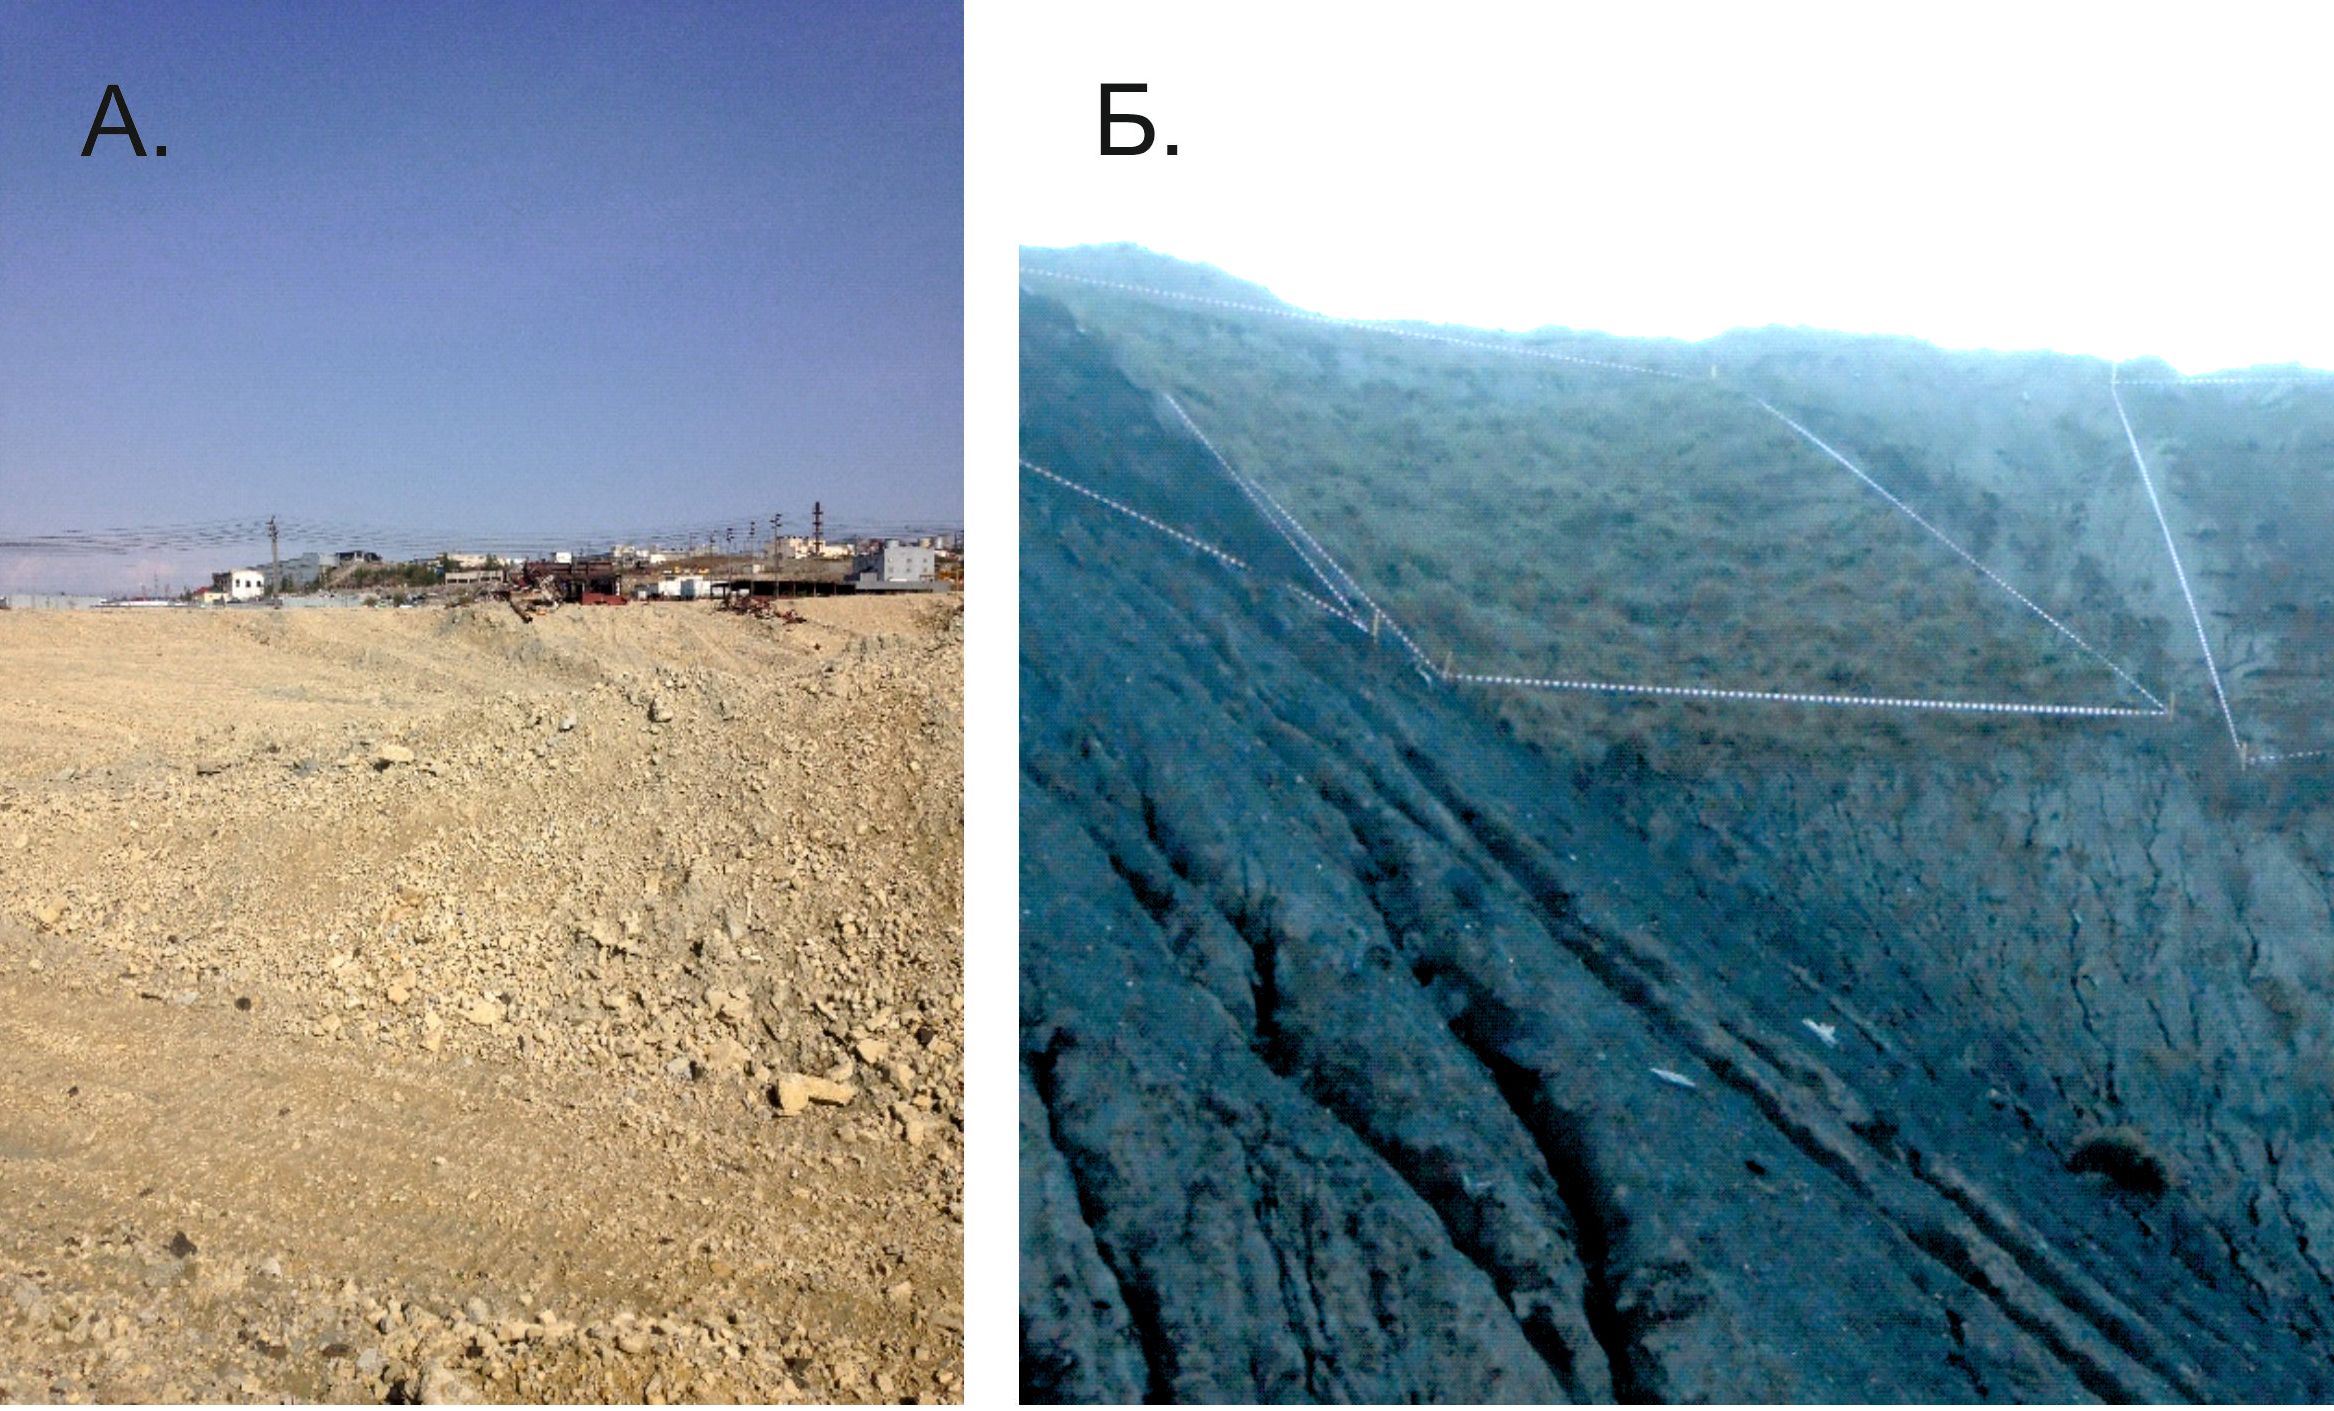
\includegraphics[width=0.9\textwidth]{authors/nekiforov-fig1.jpg}
  \end{center}
  \caption{Поверхность отвала пустых пород карьера <<Айхал>> (А) и откос отвала угольного разреза <<Кангаласский>> (Б)}
  \label{fig:nekiforov-fig1}
\end{figure}

\begin{figure}
  \begin{center}
    
\includegraphics[width=0.9\textwidth]{authors/nekiforov-fig2.jpg}
  \end{center}
  \caption{Опытно-экспериментальная площадка, накрытая старикой:
  А~--- отвал пустых пород карьера <<Айхал>>; Б~-- отвал угольного разреза <<Кангаласский>>}
  \label{fig:nekiforov-fig2}
\end{figure}

\begin{figure}
  \begin{center}
    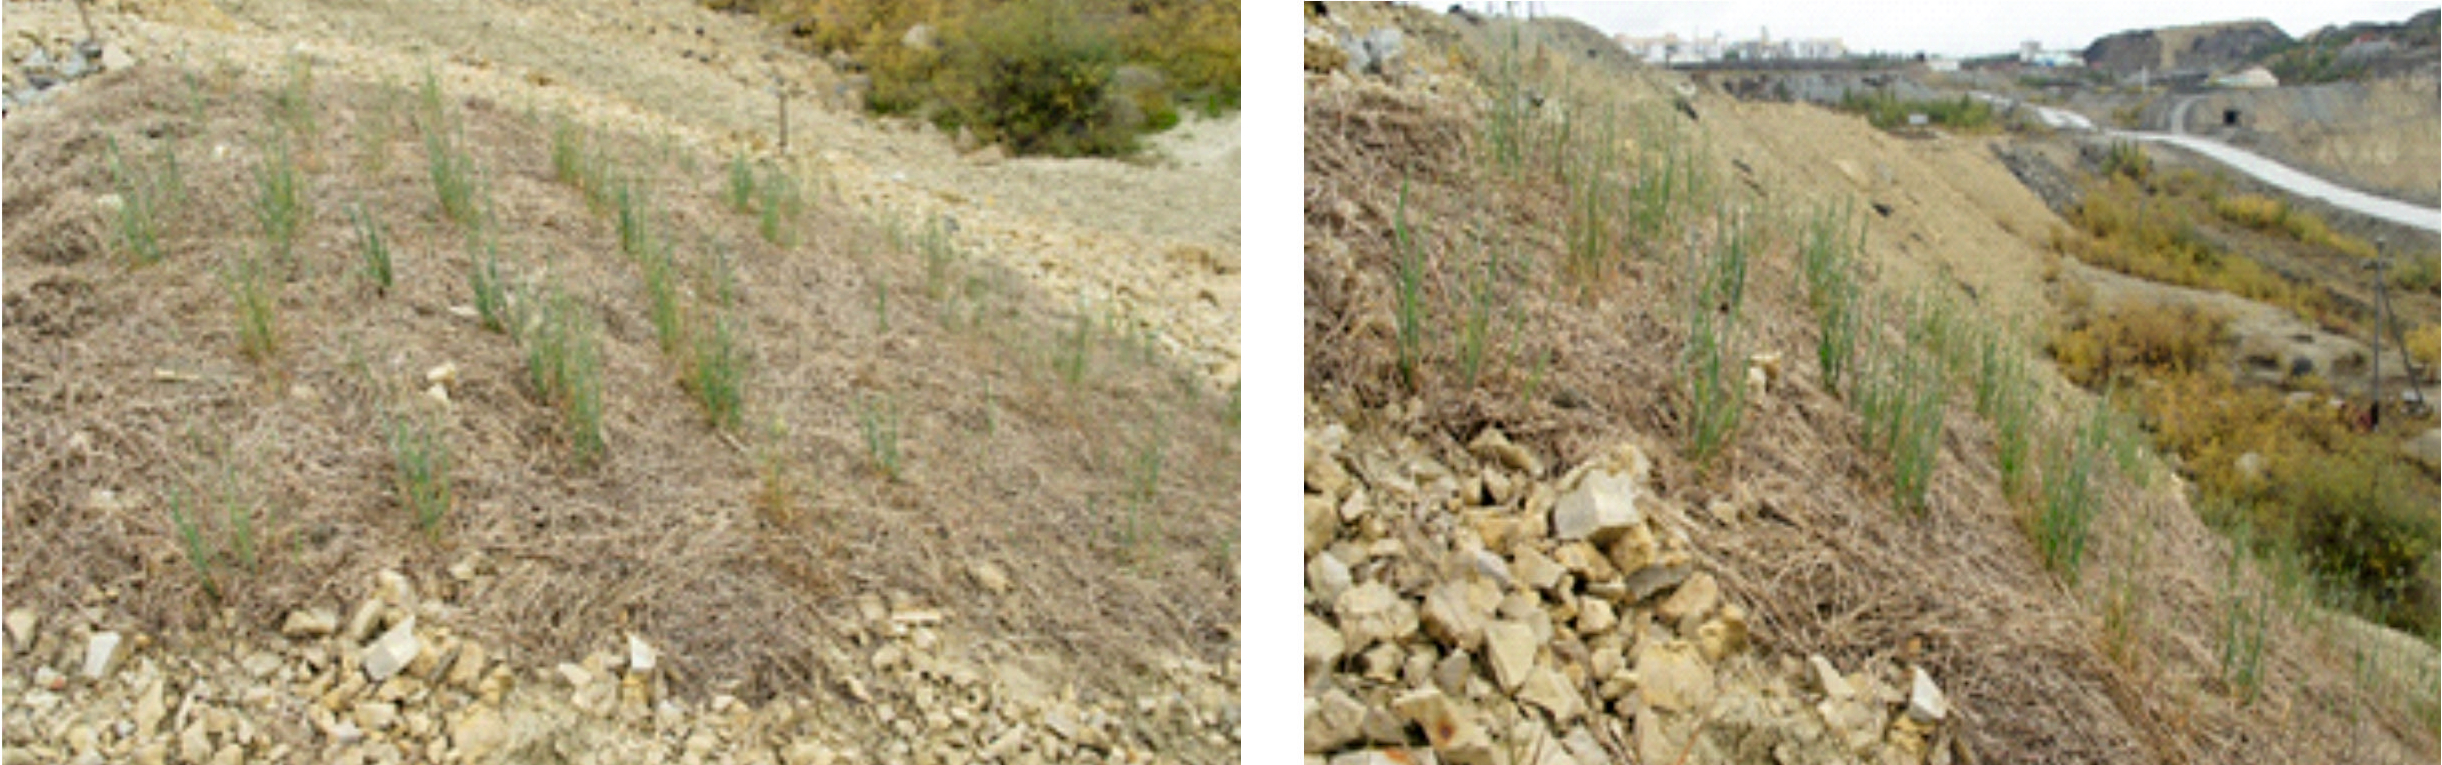
\includegraphics[width=0.9\textwidth]{authors/nekiforov-fig3.jpg}
  \end{center}
  \caption{Опытно-экспериментальная площадка с применением старики (ветоши) на отвале пустых пород карьера <<Айхал>>}
  \label{fig:nekiforov-fig3}
\end{figure}


На опытно-экспериментальной площадке в отвале угольного разреза <<Кангаласский>> среднее проективное покрытие травостоя на май месяц наблюдений составило 40--50\,\%, средняя высота 10--15\,см (май), видны всходы злаков и разнотравья. При наблюдении в июне месяце общее проективное покрытие составило 50-60\,\%, всхожесть высеянных трав составило 80\,\%, видовой состав насчитывалось до 7 видов (рис. 4).

\begin{figure}
  \begin{center}
    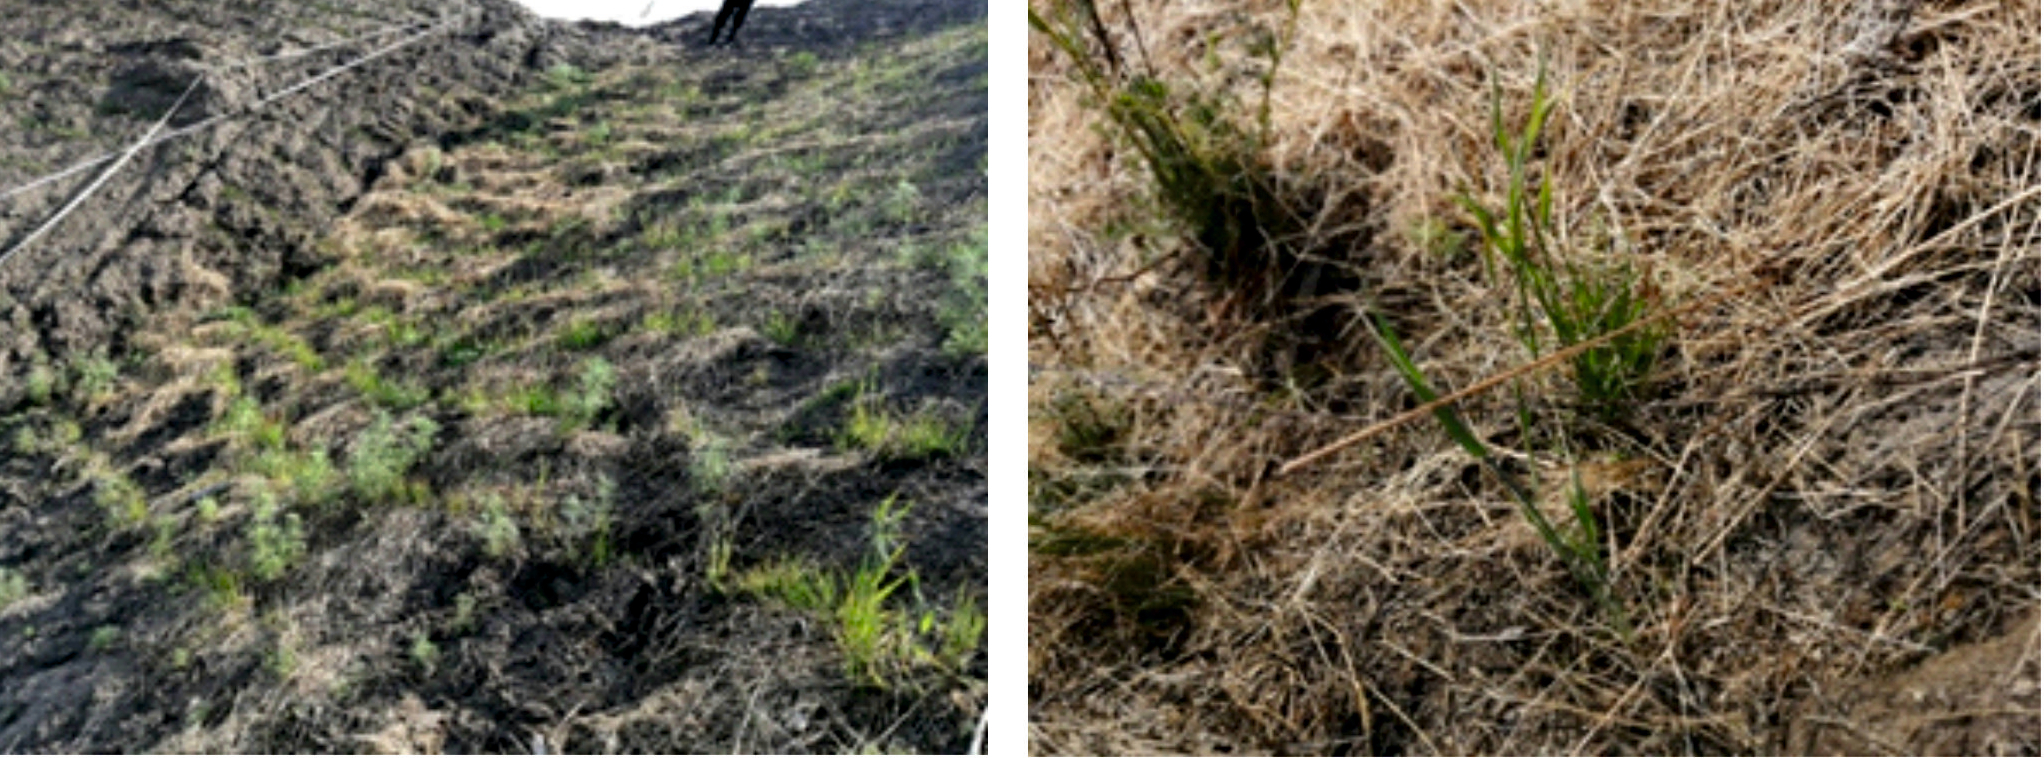
\includegraphics[width=0.9\textwidth]{authors/nekiforov-fig4.jpg}
  \end{center}
  \caption{Опытно-экспериментальная площадка с применением старики (ветоши) на отвале угольного разреза <<Кангаласский>>}
  \label{fig:nekiforov-fig4}
\end{figure}


Способ показал с перспективной стороны для внедрения в промышленных масштабах с учётом разработки технологий сбора и применения на более больших территориях. Применения старики в биологической рекультивации отвалов алмазодобычи в республике проведены впервые. В других странах этот метод применяют для других целей и в небольших объёмах только для огородов, теплицах, чаще всего в частном секторе. К применению нетрадиционного способа подтолкнуло именно условие нашего региона~--- это суровые климатические условия, экономическая целесообразность, отсутствие на данной территории потенциально плодородного слоя для отсыпки отвалов.
\clearpage
В других регионах России и мира отсыпка потенциально плодородным слоем нарушенных земель при биологической рекультивации обязательна. В нашей ситуации отсыпка плодородного слоя фактически невозможна в связи с их отсутствием, или экономической нецелесообразности их отсыпки, учитывая характер подстилающих пород траппового характера.

\textbf{Выводы}

В результате опытно-экспериментальных работ по биологической рекультивации отвалов карьера <<Айхал>> и отвалов угольного разреза <<Кангаласский>> способ применения старики (ветоши) показал наиболее эффективные результаты.

В последующем мало затратный способ можно, осуществлять повсеместно как укрывной материал без привязки к сезонным изменениям, а также в условиях отсутствия регулярного полива старика (ветошь) может, послужит задерживанием влаги и защитным слоем для всхожести семян, а при разложении питательным субстратом для роста и питания растений.

\begin{thebibliography}{99}

\bibitem{}
\BibAuthor{Лебедева\,H.\,A., Лонкунова\,А.\,Я.} Биологическая рекультивация земель, нарушенных при добыче алмазов в Якутии // Растения и промышленная среда.~--- Свердловск, 1990.~--- 71--75\,с.

\bibitem{}
ГОСТ Р 57446-2017. Наилучшие доступные технологии. Рекультивация нарушенных земель и земельных участков. Восстановление биологического разнообразия (с Поправкой).~--- Москва: Стандартинформ, 2019.~--- 47\,с.

\bibitem{}
\BibAuthor{Миркин\,Б.\,М.} Методика указания для практикума по классификации растительности методом Браун-Бланке.~--- Уфа, 1985.~--- 32\,с.
\end{thebibliography}
